% !TEX TS-program = pdflatex
% !TEX encoding = UTF-8 Unicode

% This is a simple template for a LaTeX document using the "article" class.
% See "book", "report", "letter" for other types of document.

\documentclass[11pt]{article} % use larger type; default would be 10pt

\usepackage[utf8]{inputenc} % set input encoding (not needed with XeLaTeX)

%%% Examples of Article customizations
% These packages are optional, depending whether you want the features they provide.
% See the LaTeX Companion or other references for full information.

%%% PAGE DIMENSIONS
\usepackage{geometry} % to change the page dimensions
\geometry{a4paper} % or letterpaper (US) or a5paper or....
% \geometry{margin=2in} % for example, change the margins to 2 inches all round
% \geometry{landscape} % set up the page for landscape
%   read geometry.pdf for detailed page layout information

\usepackage{graphicx} % support the \includegraphics command and options

\usepackage[parfill]{parskip} % Activate to begin paragraphs with an empty line rather than an indent

%%% PACKAGES
\usepackage{booktabs} % for much better looking tables
\usepackage{array} % for better arrays (eg matrices) in maths
\usepackage{paralist} % very flexible & customisable lists (eg. enumerate/itemize, etc.)
\usepackage{verbatim} % adds environment for commenting out blocks of text & for better verbatim
\usepackage{subfig} % make it possible to include more than one captioned figure/table in a single float
% These packages are all incorporated in the memoir class to one degree or another...

%%% HEADERS & FOOTERS
\usepackage{fancyhdr} % This should be set AFTER setting up the page geometry
\pagestyle{fancy} % options: empty , plain , fancy
\renewcommand{\headrulewidth}{0pt} % customise the layout...
\lhead{}\chead{}\rhead{}
\lfoot{}\cfoot{\thepage}\rfoot{}

%%% SECTION TITLE APPEARANCE
\usepackage{sectsty}
\allsectionsfont{\sffamily\mdseries\upshape} % (See the fntguide.pdf for font help)
% (This matches ConTeXt defaults)

%%% ToC (table of contents) APPEARANCE
\usepackage[nottoc,notlof,notlot]{tocbibind} % Put the bibliography in the ToC
\usepackage[titles,subfigure]{tocloft} % Alter the style of the Table of Contents
\renewcommand{\cftsecfont}{\rmfamily\mdseries\upshape}
\renewcommand{\cftsecpagefont}{\rmfamily\mdseries\upshape} % No bold!

%%% END Article customizations

%%% The "real" document content comes below...

\title{Thesis Progress Report 4}
\author{Aytar Akdemir \\ 150170115}
%\date{} % Activate to display a given date or no date (if empty),
         % otherwise the current date is printed 

\begin{document}
\maketitle

\section{Naessens' Formalization Methodology}

Formalization is a collection of specifications that will define a system.
While implementing a system, the rules of formalization will be used.
Defining the formal specifications, comes after the requirements analysis and before the implementation. 
For the most abstract formalism, A Flow Graph is utilised.



In [Cite naessens], Naessens divides conceptual design to three phases:

\begin{itemize}
\item Order constraints and multiplicity constraints
\item Authentication and authorization constraints
\item Control measures
\end{itemize}

Flow chart are used for order constraints and Petri nets are used for the authorization constraints. 
A Linkability Graph is used for modelling control measures.

In the article, they transform the Petri Net into a Flow Graph and the Linkability Graph into a Petri Net.


\subsection{Order and Multiplicity Constraints}

Order and Multiplicity Constraints are basically the rules on the order of the actions that can be performed and the number of times those actions can be performed. 
For example a user cannot remove a file before creating that file first. 
As an example of the multiplicity constraint, file creation can be performed multiple times denoted by ``*''; file deletion can only be performed once on a file, which is denoted by ``1''. 

An example of a flow graph is given below.

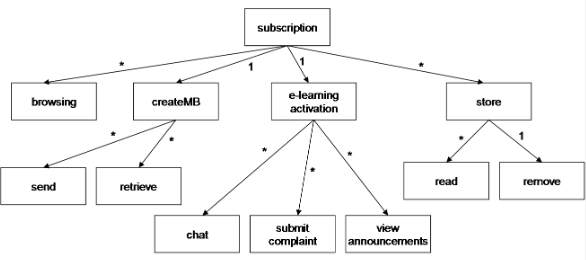
\includegraphics[width=\textwidth]{flow}

\subsection{Petri Net Representation}

In Petri Net, each right is represented with a token.
Tokens are stored in Places and each Action has Places before and after it.
If there is at least one token in the Places that point to the Action, Action can be performed and the next Place is marked with a token.
Inputs to an Action might have a natural number and a condition property:
\begin{itemize}
\item Condition can further constrain if a token is accepted by the Action.
\item The natural number is the minimum number of tokens accepted.
\end{itemize}
If the output has a natural number, the specified amount of tokens will be placed to the next Place.
The condition on the output is the additional constraints that are not tied to the inputs. 

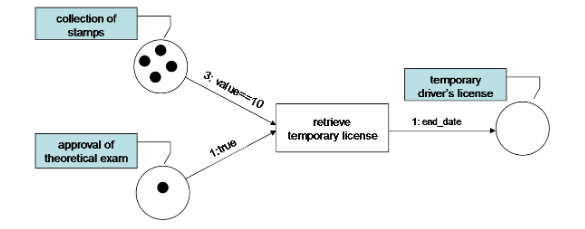
\includegraphics[width=\textwidth]{petri}

If the place after the action doesn't need to have a token, i.e. just prove it has the tokens to obtain a right, the token can be returned to the place before the action.
After the transition, the state is unchanged even though the action has been performed.

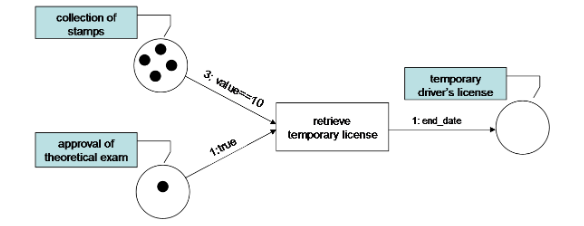
\includegraphics[width=\textwidth]{petri2}

The tokens attributes might change after the action. After the action, a mutator changes the value of the token. It is possible to have more than one transition for different conditions.

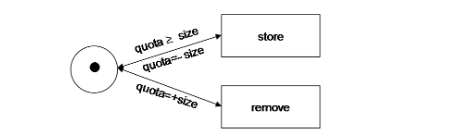
\includegraphics[width=\textwidth]{petri3}




\end{document}
